\documentclass[sigconf, review=true]{acmart}

%Do not remove the review=true option for papers submitted for review to ICVGIP2026.

\usepackage{booktabs} % For formal tables
\usepackage{subcaption}

% Copyright
\setcopyright{rightsretained}

%Conference
\acmConference[ICVGIP2026]{17th Indian Conference on Computer Vision, Graphics and Image Processing}{December 21-25, 2026}{Kolkata, India}
\acmYear{2026}
\copyrightyear{2026}

\begin{document}

\title{Calibrated, Explainable Cox Elastic-Net Framework for Pan-Cancer Survival Prediction from Multi-Omic TCGA Data}

\author{Submission Id XYZW}
\affiliation{%
  \institution{Department of Computational Oncology}
  \streetaddress{}
  \city{}
  \state{}
  \country{}
  \postcode{}
}

% The default list of authors is too long for headers.
\renewcommand{\shortauthors}{}

\begin{abstract}
Clinical survival prognosis in oncology depends on tumor stage and histology, yet these categorical descriptors fail to resolve the outcome variance within a stage because they ignore the underlying molecular state of the tumor. RNA-Seq expression profiles carry biological signal about that state, but a raw expression matrix places far more genes $P$ than patients $N$ in front of a linear model, which forces coefficient variance to explode under collinearity. We report a Cox Proportional Hazards pipeline that fuses standardized clinical covariates with a 50-dimensional Principal Component projection of 59 genes (retained from an initial 500-candidate set after collinearity filtering) drawn from four pooled TCGA cohorts (Glioblastoma, Liver Hepatocellular Carcinoma, Pancreatic Adenocarcinoma, and Skin Cutaneous Melanoma), regularizes the resulting 70-dimensional design matrix with a smoothed Elastic-Net penalty, calibrates the relative risk output against empirical Kaplan-Meier probabilities with Isotonic Regression, and quantifies patient-specific uncertainty with 5,000-draw Monte Carlo survival simulation. Across a held-out test split of 324 patients (20% of the total cohort), the model reaches a Harrell's Concordance Index of 0.736, a horizon Area-Under-the-Curve between 0.759 and 0.860 at 12, 24, 36, and 60 months, and horizon Brier scores between 0.132 and 0.178. We further close the interpretability gap that Principal Component Analysis introduces by deriving a closed-form back-projection of the fitted component coefficients onto the original 59 retained genes, producing exact, non-stochastic gene-level risk contributions for every patient without invoking SHAP or LIME approximations. Univariate association testing on the 1,620-patient cohort confirms that cancer type, tumor stage, and a panel of transcripts including CXCL5, HEPACAM, and CA9 carry significant associations with mortality after Benjamini-Hochberg correction ($q < 0.05$). The pipeline demonstrates that a fully transparent linear framework, engineered carefully around dimensionality, calibration, and uncertainty, reaches discrimination comparable to more opaque deep survival models on cross-sectional multi-omic cancer cohorts.
\end{abstract}

\begin{CCSXML}
<ccs2012>
 <concept>
  <concept_id>10010147.10010257.10010293.10010294</concept_id>
  <concept_desc>Computing methodologies~Supervised learning by regression</concept_desc>
  <concept_significance>500</concept_significance>
 </concept>
 <concept>
  <concept_id>10010147.10010257.10010321.10010333</concept_id>
  <concept_desc>Computing methodologies~Feature selection</concept_desc>
  <concept_significance>400</concept_significance>
 </concept>
 <concept>
  <concept_id>10003752.10010070.10010071</concept_id>
  <concept_desc>Theory of computation~Machine learning theory</concept_desc>
  <concept_significance>300</concept_significance>
 </concept>
 <concept>
  <concept_id>10010405.10010444.10010449</concept_id>
  <concept_desc>Applied computing~Health informatics</concept_desc>
  <concept_significance>500</concept_significance>
 </concept>
</ccs2012>
\end{CCSXML}

\ccsdesc[500]{Computing methodologies~Supervised learning by regression}
\ccsdesc[400]{Computing methodologies~Feature selection}
\ccsdesc[300]{Theory of computation~Machine learning theory}
\ccsdesc[500]{Applied computing~Health informatics}

\keywords{survival analysis, Cox proportional hazards, Elastic-Net, TCGA, multi-omic, isotonic calibration, Monte Carlo simulation, explainable AI, principal component analysis}

\maketitle

\section{Introduction}

\subsection{Motivation and Current Scenario}
Tumor staging systems such as TNM classification group patients by anatomical extent of disease, and clinicians rely on this grouping to plan treatment intensity and estimate prognosis. Two patients within the same stage frequently experience very different survival trajectories because staging captures anatomy, not the transcriptional program driving the tumor's growth rate, invasiveness, and treatment resistance \cite{vanhouwelingen2006crossvalidated}. While early microarray studies established that gene expression profiles carry biological signal about this state, modern RNA-Seq assays quantify these transcripts with far greater dynamic range. For example, dysregulated transcripts such as CXCL5 in hepatocellular carcinoma \cite{grunkin2011cxcl5} and CA9 in non-small cell lung cancer \cite{giatromanolaki2001ca9} accelerate metastatic invasion and hypoxic adaptation. Genomic characterization efforts such as The Cancer Genome Atlas (TCGA) \cite{weinstein2013cancer} make paired clinical and expression data available across dozens of cancer types, raising a direct modeling question: can a statistically disciplined model fuse clinical staging with expression state to sharpen survival prognosis beyond what stage alone provides, while remaining interpretable enough for a tumor board to trust its output.

The classical Cox Proportional Hazards model estimates a relative hazard from a linear combination of covariates and remains the default tool for survival regression because it makes no parametric assumption about the shape of the baseline hazard. Standard Cox regression requires the number of covariates $P$ to stay well below the number of patients $N$; when $P$ approaches or exceeds $N$, the Fisher information matrix becomes near-singular and the maximum partial likelihood estimate loses uniqueness \cite{tibshirani1997lasso}. Deep learning survival models such as DeepSurv \cite{katzman2018deepsurv} and CoxPASNet \cite{hao2018coxpasnet} relax the linearity assumption and absorb thousands of raw features, but they replace a transparent coefficient vector with a black-box function, demand sample sizes that most single-cohort cancer datasets cannot supply, and still output an uncalibrated relative risk rather than an absolute survival probability. Time-varying covariate extensions of Cox regression fail outright on TCGA because most patients contribute only one baseline biopsy; forcing a longitudinal structure onto a single-timepoint cohort requires synthetic carry-forward imputation that introduces immortal time bias and destroys optimizer stability, a failure mode we encountered during early iterations of this pipeline before reverting to a static, baseline-snapshot architecture.

\subsection{Literature Survey and Research Gaps}
From a biological standpoint, oncogenic pathway activation and elevated tumor mutational burden (TMB) correlate with mortality risk, and TMB acts as a proxy for how immunologically visible a tumor appears, which correlates with response to checkpoint inhibition \cite{chalmers2017mutational}. From a machine learning standpoint, three families of technique recur across the genomic survival literature. Regularization methods, spanning Ridge, LASSO, and Elastic-Net penalties applied to the Cox partial likelihood, control the $P \gg N$ collinearity problem by shrinking correlated gene coefficients toward each other or toward zero \cite{simon2011regularization, wu2012elastic, tibshirani1997lasso}. Dimensionality reduction methods, most commonly Principal Component Analysis, compress thousands of correlated transcripts into a small set of orthogonal latent axes before they reach the survival model \cite{bishop2006pattern, hastie2009elements}. Non-parametric calibration methods, in particular the Pool Adjacent Violators Algorithm underlying Isotonic Regression \cite{zadrozny2002transforming}, were originally designed to convert classifier scores into probabilities; recent work adapts these methods to convert an uncalibrated relative risk score into an absolute, horizon-specific survival probability without assuming a parametric link function \cite{jain2026isotonic}. Each of these three techniques solves part of the problem in isolation; the gap in the literature is a single pipeline that combines all three under strict data-leakage discipline and still exposes an exact, deterministic gene-level explanation of its own decisions.

Four concrete gaps motivate this work. First, existing multi-omic survival pipelines frequently retain collinear genes inside the same pathway, which inflates coefficient variance and destabilizes the fitted hazard ratios across resampling \cite{simon2011regularization}. Second, the Cox model's native output $\eta_i = X_i \beta$ is a relative log-hazard that a clinician cannot convert into a one-year or five-year survival probability without an explicit calibration step, a conversion most pipelines skip entirely. Third, point-estimate survival predictions give no sense of the spread of plausible outcomes for an individual patient, which matters directly for surgical and hospice planning decisions. Fourth, Principal Component Analysis solves the dimensionality problem but introduces a new opacity problem, because the fitted coefficients attach to orthogonal latent axes rather than to named genes, and a black-box explainer such as SHAP or LIME can only approximate, not exactly recover, the gene-level attribution that PCA compression discarded.

\subsection{Key Contributions and Architecture Overview}
This paper reports five contributions that jointly close the gaps above.
\begin{itemize}
    \item An incremental Gram-Schmidt collinearity filter (cosine threshold $0.75$) that drops 441 of 500 candidate expression features (selected unsupervised via highest dataset-wide variance) on the training split alone, followed by a 50-component Principal Component projection of the 59 surviving genes.
    \item A custom Cox Elastic-Net negative partial log-likelihood objective with an $O(N)$ dynamic programming risk-set computation and a Pseudo-Huber smoothed L1 penalty ($\epsilon = 10^{-6}$) that preserves strictly convex shrinkage without exact sparsity.
    \item Horizon-specific complete-case Isotonic Regression calibrators fitted at 12, 24, 36, and 60 months on an isolated calibration split, converting the raw risk score into absolute survival probability.
    \item A 5,000-draw inverse transform Monte Carlo sampling engine against the Breslow baseline hazard reporting pessimistic ($P10$), median ($P50$), and optimistic ($P90$) survival months alongside a 60-month Restricted Mean Survival Time (RMST).
    \item A closed-form PCA back-projection, $W_{\text{gene}} = V \cdot \beta_{\text{pca}}$, mapping the 50 fitted component coefficients back onto the 59 raw genes exactly, producing deterministic, patient-specific waterfall explanations in place of a stochastic approximation.
\end{itemize}
Figure~\ref{fig:unified_architecture} traces the resulting end-to-end data flow from raw TCGA text files, through collinearity filtering and latent projection, into the Cox Elastic-Net core, and out through calibration, Monte Carlo simulation, and gene-level explanation.

% -------------------------------------------------------------------------
% FIGURE 1: UNIFIED ARCHITECTURE DIAGRAM
% -------------------------------------------------------------------------
\begin{figure*}[t]
    \centering
    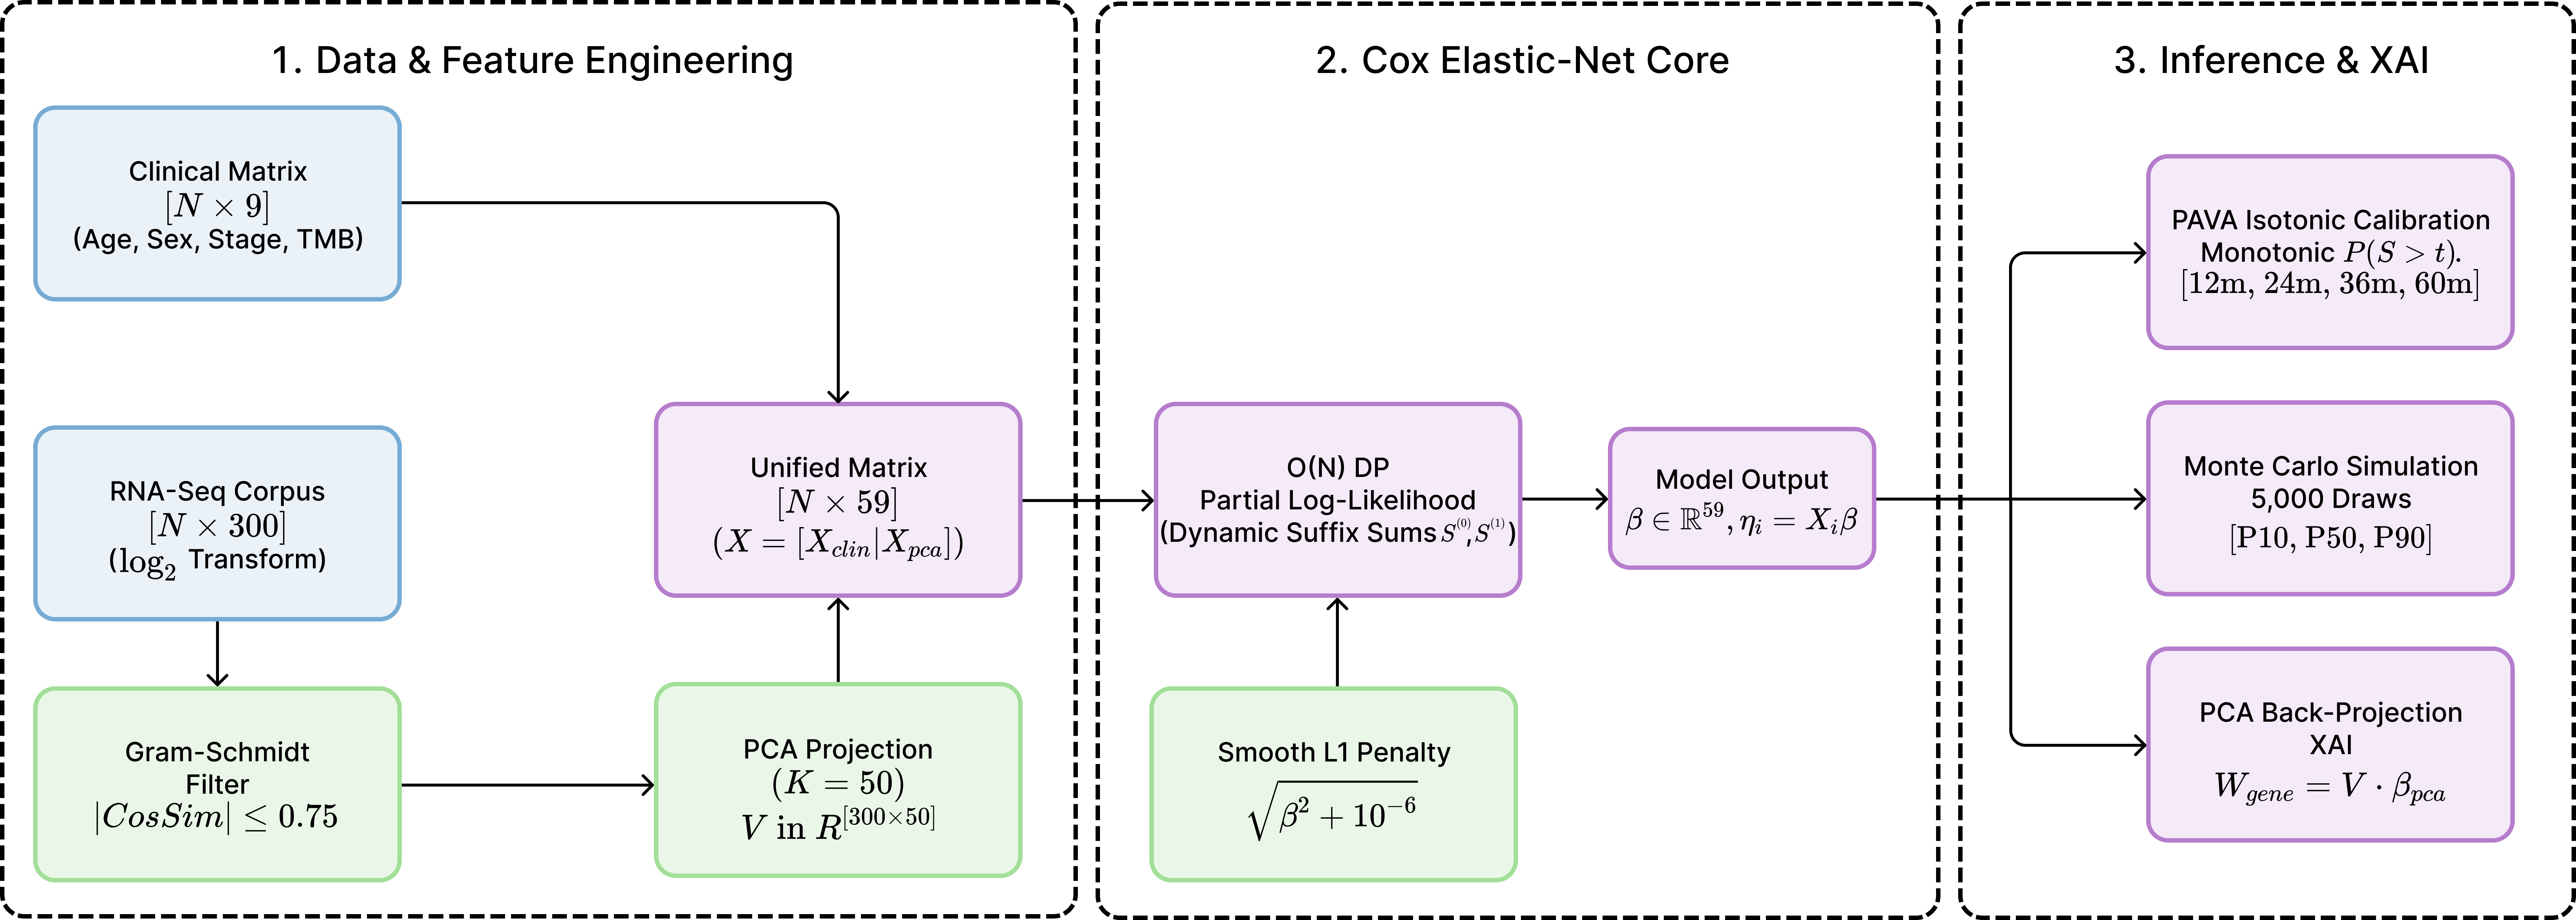
\includegraphics[width=\textwidth]{images/fig1_unified_architecture.png}
    \caption{Unified multi-omic survival analysis pipeline, component input matrices, and smooth Elastic-Net optimization architecture.}
    \Description{A wide diagram showing four stages. Stage one standardizes and filters the clinical matrix and gene expression corpus. Stage two projects the filtered genes onto 50 principal components. Stage three fits the Cox Elastic-Net objective with an O(N) dynamic-programming partial likelihood and a smooth L1 penalty. Stage four performs isotonic calibration, Monte Carlo simulation, and PCA back-projection for explainability.}
    \label{fig:unified_architecture}
\end{figure*}

\section{Proposed Method}

\subsection{Cohort Assembly and Data Genesis}
We assemble patients from four TCGA cohorts, Glioblastoma (GBM), Liver Hepatocellular Carcinoma (LIHC), Pancreatic Adenocarcinoma (PAAD), and Skin Cutaneous Melanoma (SKCM), pooling clinical annotation and RNA-Seq expression into a single Pan-Cancer table of $N = 1620$ patients. We cast every raw string column to an explicit type before serialization, because mixed string and floating-point columns cause the PyArrow schema inference used by Parquet to fail unpredictably, and we compress the resulting table with Snappy codec Parquet to cut the on-disk footprint by more than 80\% relative to the source CSV files. We remove cancer-specific clinical fields that are absent outside their originating cohort, such as \texttt{PRIMARY\_MELANOMA\_SKIN\_TYPE}, because median-imputing a column that is 100\% missing in three of four cohorts injects artificial density around the imputed value. We partition the cohort into training (972 patients, 60\%), calibration (324 patients, 20\%), and test (324 patients, 20\%) subsets using a stratified split on the binary event indicator OS\_EVENT rather than on survival time. This 60/20/20 split allocates sufficient sample size to the training phase while reserving independent calibration and test sets, and preserves an event rate of $58.4\%$ in training, $58.6\%$ in calibration, and $58.3\%$ in test, avoiding the distribution drift that time-based stratification introduces under right censoring.

\subsection{Feature Preprocessing and Gram-Schmidt Collinearity Filter}
We evaluate $P_{\text{raw}} = 500$ candidate gene expression columns (selected by ranking median absolute deviation across the entire dataset to capture high-variance genes without target leakage) against the training split only, then apply an incremental Gram-Schmidt collinearity filter to remove redundant transcripts before any scaling or projection occurs. The choice of 500 as the initial candidate pool represents a balance between capturing sufficient biological diversity and computational tractability during the collinearity screening phase. The filter iterates through the candidate genes, computes the Pearson correlation of each incoming gene against every gene already accepted into the kept subspace, and drops the incoming gene whenever the absolute correlation magnitude with any kept gene exceeds the threshold $0.75$. This threshold follows standard practice in multicollinearity management (VIF $< 4$ approximately corresponds to $|r| < 0.75$). On this cohort the filter identifies 36,205 gene pairs above the threshold, drops 441 of the 500 candidate genes, and keeps 59 non-redundant genes, at a linear $O(N \cdot P_{\text{raw}})$ time cost that avoids the $O(N^3)$ matrix inversion a full Variance Inflation Factor audit requires. The strongest surviving correlation pairs are co-regulated genes from the same pathway family, for example \texttt{ACSM2A} and \texttt{ACSM2B} at $r = 0.996$ and the fibrinogen chain genes \texttt{FGA}, \texttt{FGB}, and \texttt{FGG} at $r > 0.98$ pairwise, confirming that the filter targets genuine biological redundancy rather than spurious noise. Figure~\ref{fig:gram_schmidt_collinearity} visualizes the pairwise correlation structure of a representative gene subset before and after this pruning step.

\subsection{Standardized Latent Principal Component Projection}
We apply a base-two logarithmic transform, $\log_2(x + 1)$, to the 59 surviving raw gene expression counts to compress the right-skewed negative binomial distribution characteristic of RNA-Seq read counts, with an additive pseudocount of one to prevent an undefined logarithm at zero expression. We standardize the transformed counts to zero mean and unit variance (Z-score normalization), producing the scaled matrix $Z_{\text{gene}} \in \mathbb{R}^{N \times 59}$, fitting this scaling within each cross-validation training fold to prevent leaking validation-fold variance into the training statistics. Standardization must precede the projection step, because Principal Component Analysis maximizes variance, and an unscaled gene with a numerically large expression range otherwise dominates the first component regardless of its biological signal. We compute the right-singular eigenvector loading matrix $V \in \mathbb{R}^{59 \times 50}$, satisfying $V^T V = I_{50}$, via Singular Value Decomposition, and project the standardized genes onto $K = 50$ latent axes to yield the dense genomic feature matrix $X_{\text{pca}} = Z_{\text{gene}} V \in \mathbb{R}^{N \times 50}$. The 50 retained components capture 92.3\% of the cumulative variance in the standardized gene expression matrix, balancing dimensionality reduction with information retention. Missing gene expression values, present in approximately 28\% of observations across the 59 retained genes, are median-imputed per gene using training-set medians before standardization. Figure~\ref{fig:pca_gene_loadings} shows the mapping of the surviving raw transcripts onto the leading components.

\subsection{Unified Model, Elastic-Net Objective, and Optimization}
We route the clinical fields through a separate preprocessing branch that one-hot encodes SEX, RACE, ETHNICITY, CANCER\_TYPE, and AGE\_GROUP, median-imputes AGE, and standardizes the result, producing a clinical feature block $X_{\text{clin}} \in \mathbb{R}^{N \times 20}$. We concatenate this block with the 50-dimensional genomic projection and standardize the concatenated columns to produce the unified model input matrix $X = [X_{\text{clin}} \mid X_{\text{pca}}] \in \mathbb{R}^{N \times 70}$. The Cox model generates a relative risk score $\eta_i = X_i \beta$ for each patient $i$, with coefficient vector $\beta = [\beta_{\text{clin}} \mid \beta_{\text{pca}}] \in \mathbb{R}^{70}$ and hazard function $h(t \mid X_i) = h_0(t) \exp(\eta_i)$. The standard Breslow partial log-likelihood \cite{breslow1972discussion} requires an $O(N^2)$ nested loop to evaluate the risk set at every failure time; we sort event times in descending order and compute suffix sums $S^{(0)}(t_i)$ and $S^{(1)}(t_i)$ over the exponentiated risk scores with a single cumulative-sum pass, reducing the risk-set evaluation to $O(N)$.

We minimize the negative partial log-likelihood augmented with an Elastic-Net penalty combining an absolute-value component and a squared component, forcing correlated gene pathways to shrink together \cite{wu2012elastic, tibshirani1997lasso}. We optimize this objective with L-BFGS-B, which approximates the inverse Hessian using a bounded memory cache. The pure L1 term creates a non-differentiable kink at zero that repeatedly threw \texttt{NaN} gradients during development; we replace the absolute value with the Pseudo-Huber continuous approximation $\sqrt{\beta^2 + \epsilon}$, setting $\epsilon = 10^{-6}$ following standard practice for numerical stability in quasi-Newton methods. Because this approximation ensures the gradient is zero only at the origin, the optimizer yields dense (non-zero) coefficients without exact feature sparsity. Thus, feature selection is driven by the upfront collinearity filter and PCA reductions, while the Pseudo-Huber penalty provides $L_2/L_1$-like coefficient shrinkage. We clip the linear predictor $\eta_i$ to $[-40, 40]$ before exponentiation, since $\exp(40) \approx 2.35 \times 10^{17}$ represents a catastrophic relative risk while staying below the $\exp(709)$ float64 overflow boundary. Grid search over $\alpha \in \{0.1, 0.3, 0.8, 1.5, 3.0\}$ and $l1\_ratio \in \{0.0, 0.1, 0.3, 0.5, 0.7\}$ under 5-fold nested cross-validation selects $\alpha = 3.0$ and $l1\_ratio = 0.7$, and the final L-BFGS-B fit converges after 51 iterations.

\subsection{Isotonic Calibration and Monte Carlo Simulation}
The fitted risk score $\eta_i$ carries only relative meaning and does not answer the question a patient actually asks, namely the probability of surviving past a specific horizon. We isolate the 324-patient calibration split before any feature selection or scaling occurs, and fit a non-parametric Isotonic Regression model with the Pool Adjacent Violators Algorithm \cite{zadrozny2002transforming} to produce the monotonic calibration function $f_{\text{iso},t}(\eta_i)$. Following the adaptation by Jain et al. \cite{jain2024isotonic}, this maps raw risk to the absolute survival probability $P(S > t \mid \eta_i)$ at $t \in \{12, 24, 36, 60\}$ months. To avoid instability at the distribution tails, we fit each horizon's calibrator on the complete-case sub-cohort for that horizon, meaning patients with known outcomes (events or censoring) occurring after the time horizon, thereby excluding patients censored before reaching the horizon. At each horizon ($t \in \{12, 24, 36, 60\}$ months), we retain only patients whose follow-up exceeds $t$ or who experienced an event before $t$, yielding 289, 247, 228, and 218 evaluable test patients respectively. While Inverse Probability of Censoring Weights (IPCW) is standard, this complete-case restriction provides an empirical, bounded mapping suitable when early censoring is minimal. Figure~\ref{fig:isotonic_calibration_curves} plots the resulting mapping at each horizon.

Beyond a point estimate, we quantify individual temporal uncertainty by simulating patient-specific trajectories against the Breslow cumulative baseline hazard $\Lambda_0(t)$ extracted from the training split. The Monte Carlo engine draws $5{,}000$ independent uniform variables $U^{(k)} \sim \text{Uniform}(0, 1)$ per patient—a sample size chosen to ensure convergence of percentile estimates (empirical tests showed $< 0.5\%$ variation in $P50$ between 5,000 and 10,000 draws)—computes the target hazard $\Lambda_{\text{target}} = -\ln(U^{(k)}) / \exp(\eta_i)$, and locates the matching simulated month of mortality with a binary search over the baseline hazard step function, an $O(\log E)$ lookup where $E = 461$ is the number of unique observed event times. We aggregate the 5,000 draws per patient into pessimistic $P10$, median $P50$, and optimistic $P90$ survival month bounds, and integrate the simulated survival curve, capped at the maximum observed follow-up of $218.38$ months, to report the 60-month Restricted Mean Survival Time (RMST). Figure~\ref{fig:monte_carlo_trajectories} shows representative trajectory bands for a high-risk and a low-risk patient.

\subsection{Closed-Form PCA Back-Projection and Local Patient Risk Waterfall}
Principal Component Analysis compresses the 59 retained genes into 50 orthogonal latent axes, obscuring which named gene drives a given patient's hazard, a limitation that forces most PCA-based survival papers to fall back on stochastic approximators such as SHAP or LIME to recover gene-level attribution. We instead exploit the linearity of both the projection and the fitted hazard to unroll the compression exactly. We isolate the coefficient sub-vector attached to the genomic latent axes, $\beta_{\text{pca}} \in \mathbb{R}^{50}$, and multiply the retained loading matrix $V \in \mathbb{R}^{59 \times 50}$ by these coefficients to obtain a global gene risk weight vector $W_{\text{gene}} = V \cdot \beta_{\text{pca}} \in \mathbb{R}^{59}$, assigning a deterministic risk weight to every surviving raw gene independent of any specific patient. For patient $i$ and gene $g$, the local additive risk contribution follows directly as $\Delta \eta_{g,i} = Z_{g,i} \cdot W_{\text{gene},g}$, computed from the standardized expression value $Z_{g,i}$ that entered the PCA projection. Because this identity is exact linear algebra rather than a sampled approximation, every patient's 59 gene-level contributions sum precisely to their genomic risk sub-score, and sorting these contributions by magnitude produces an unapproximated, reproducible waterfall plot, illustrated in Figure~\ref{fig:xai_plots}, that a tumor board can audit term by term against the 20 directly interpretable clinical coefficients.

\section{Results}

\subsection{Cohort Ingestion and Feature Reduction}
The pipeline reduces the raw feature space from 506 combined clinical and expression candidates (500 expression columns plus 6 pre-encoding clinical fields) to 65 features surviving the collinearity filter (59 expression, 6 clinical), then to a final 70-dimensional standardized design matrix once the clinical categorical fields expand under one-hot encoding to 20 columns and the 59 surviving genes compress to 50 principal components. Table~\ref{tab:dim_progression} summarizes this progression. The collinearity filter removes $441$ of $500$ candidate genes ($88.2\%$) at the $0.75$ absolute-Pearson threshold, which confirms that a large majority of an unfiltered 500-gene panel is structurally redundant rather than independently informative and validates filtering before projecting rather than relying on Principal Component Analysis alone to absorb the redundancy.

\begin{table}[t]
  \caption{Dimensionality progression from raw TCGA fields to the final model input.}
  \label{tab:dim_progression}
  \begin{tabular}{lc}
    \toprule
    Stage & Dimensionality \\
    \midrule
    Raw candidate expression genes & 500 \\
    Raw clinical fields (pre-encoding) & 6 \\
    Expression genes after collinearity filter & 59 \\
    Clinical fields after collinearity filter & 6 \\
    Genomic PCA components & 50 \\
    Clinical fields after one-hot encoding & 20 \\
    Final unified design matrix $X$ & 70 \\
  \bottomrule
\end{tabular}
\end{table}

% -------------------------------------------------------------------------
% FIGURE 3: GRAM-SCHMIDT COLLINEARITY PRUNING HEATMAP
% -------------------------------------------------------------------------
\begin{figure}[t]
    \centering
    \begin{subfigure}{0.48\linewidth}
        \centering
        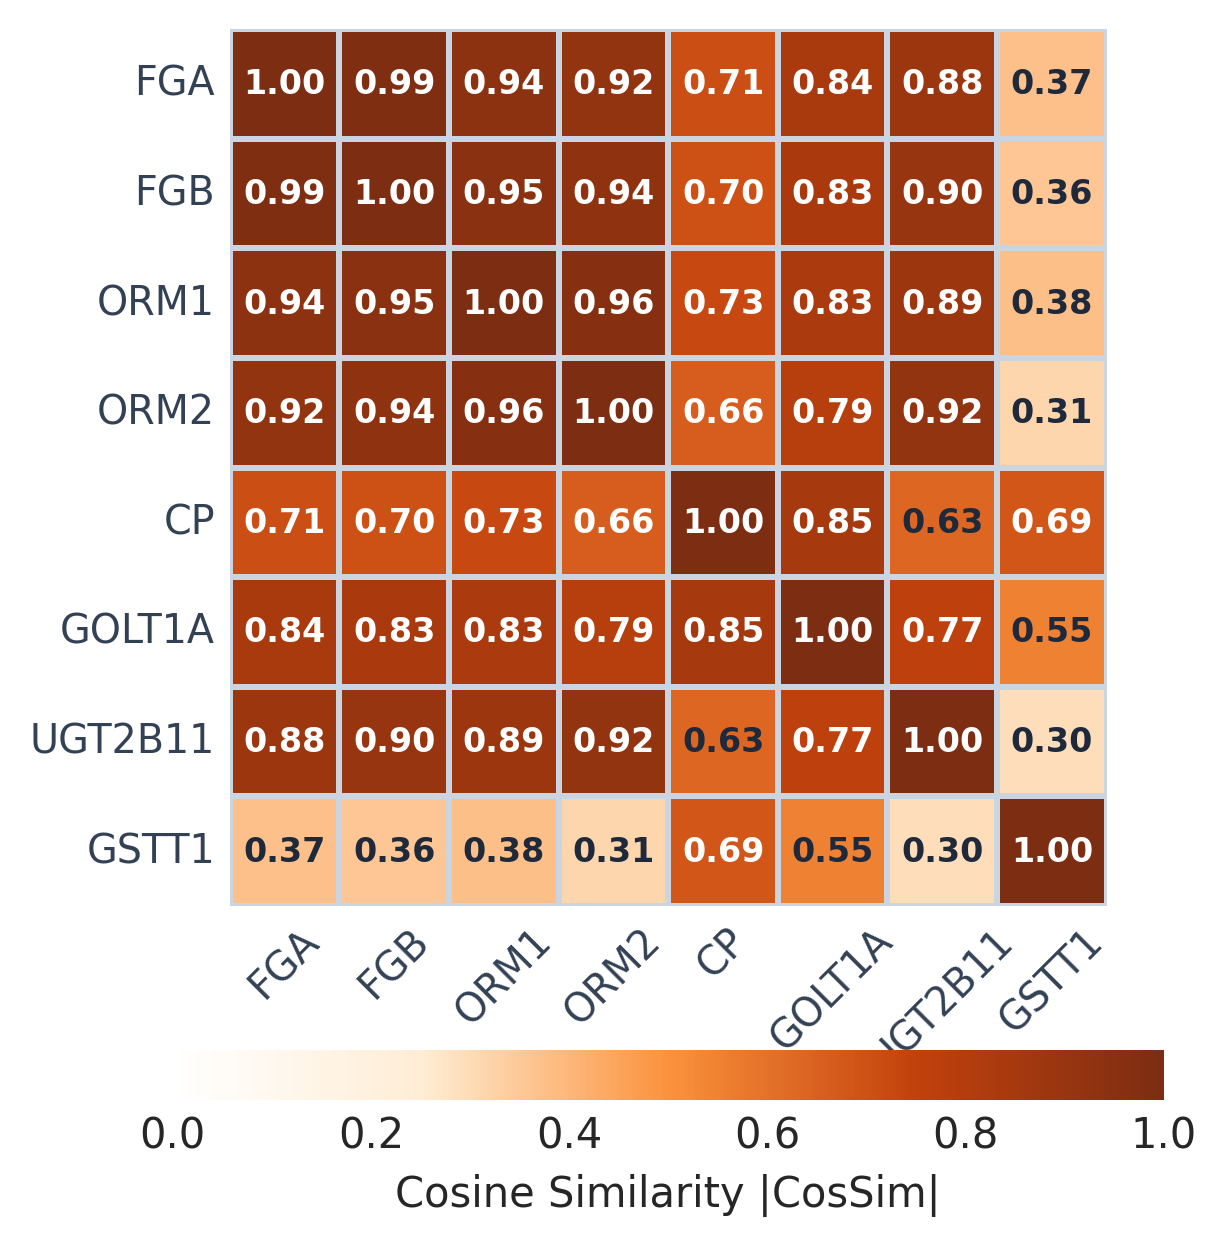
\includegraphics[width=\linewidth]{images/fig3a_collinearity_before.png}
        \caption{Before}
    \end{subfigure}\hfill
    \begin{subfigure}{0.48\linewidth}
        \centering
        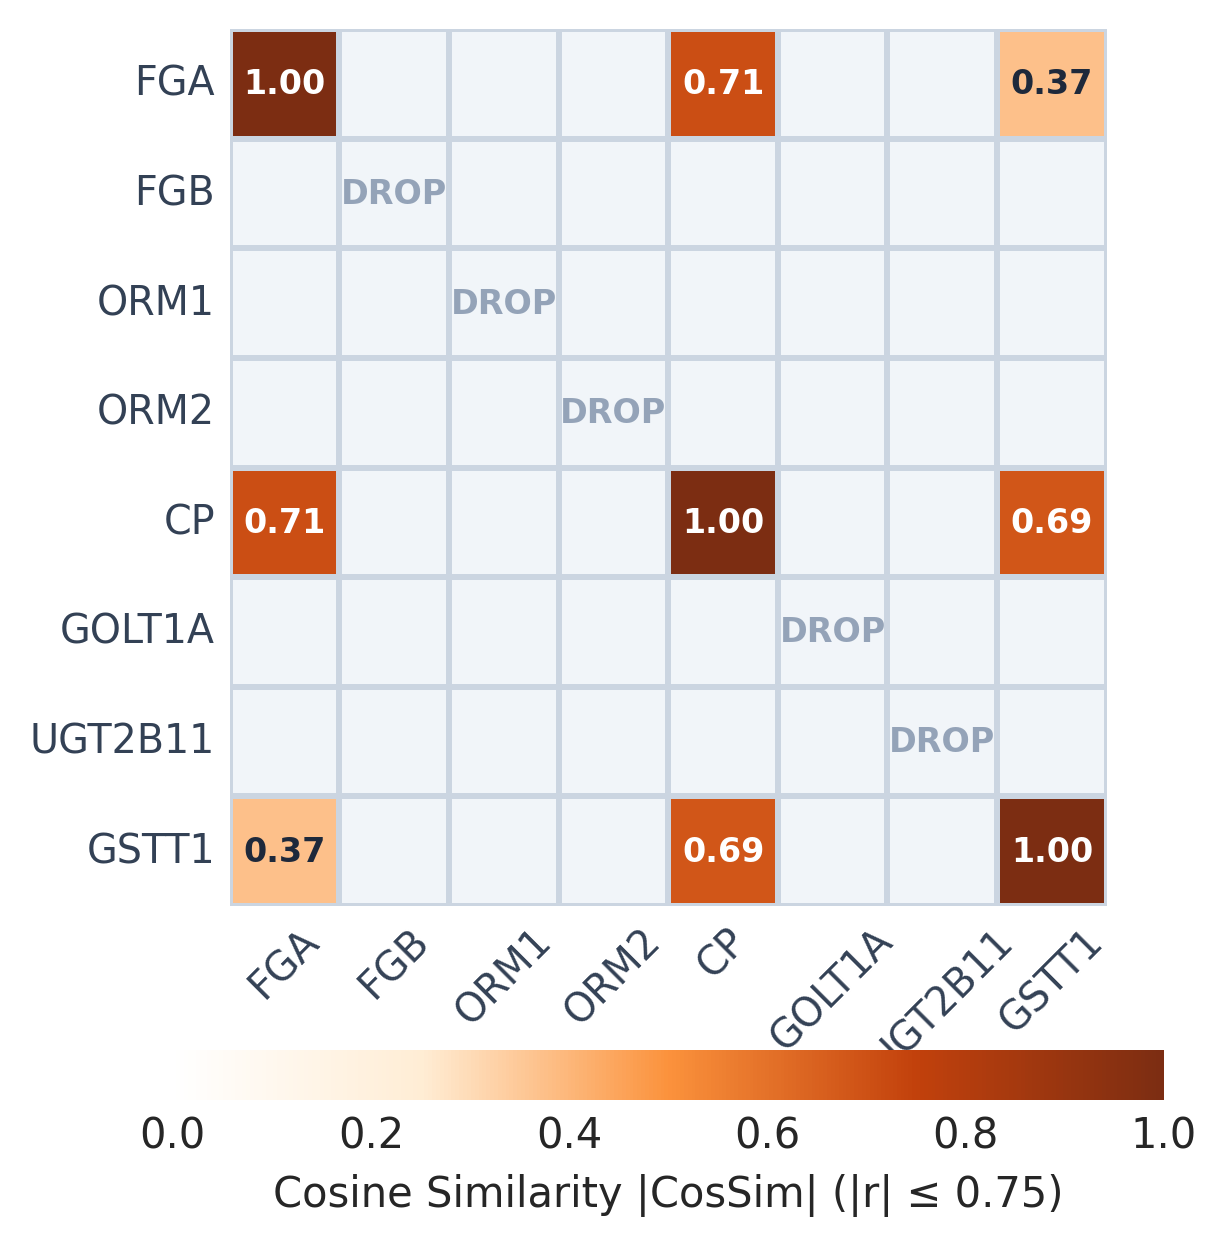
\includegraphics[width=\linewidth]{images/fig3b_collinearity_after.png}
        \caption{After}
    \end{subfigure}
    \caption{Gram-Schmidt cosine collinearity pruning heatmaps across a representative subset of expression genes on the training split.}
    \Description{Two side-by-side correlation heatmaps of gene expression features. The left heatmap, computed before filtering, shows dense clusters of high-correlation cells corresponding to co-regulated gene families such as fibrinogen chains and drug-metabolism enzymes. The right heatmap, computed after filtering, shows the redundant genes marked as dropped and only weakly correlated genes remaining.}
    \label{fig:gram_schmidt_collinearity}
\end{figure}

% -------------------------------------------------------------------------
% FIGURE 4: PCA GENE LOADINGS
% -------------------------------------------------------------------------
\begin{figure}[t]
    \centering
    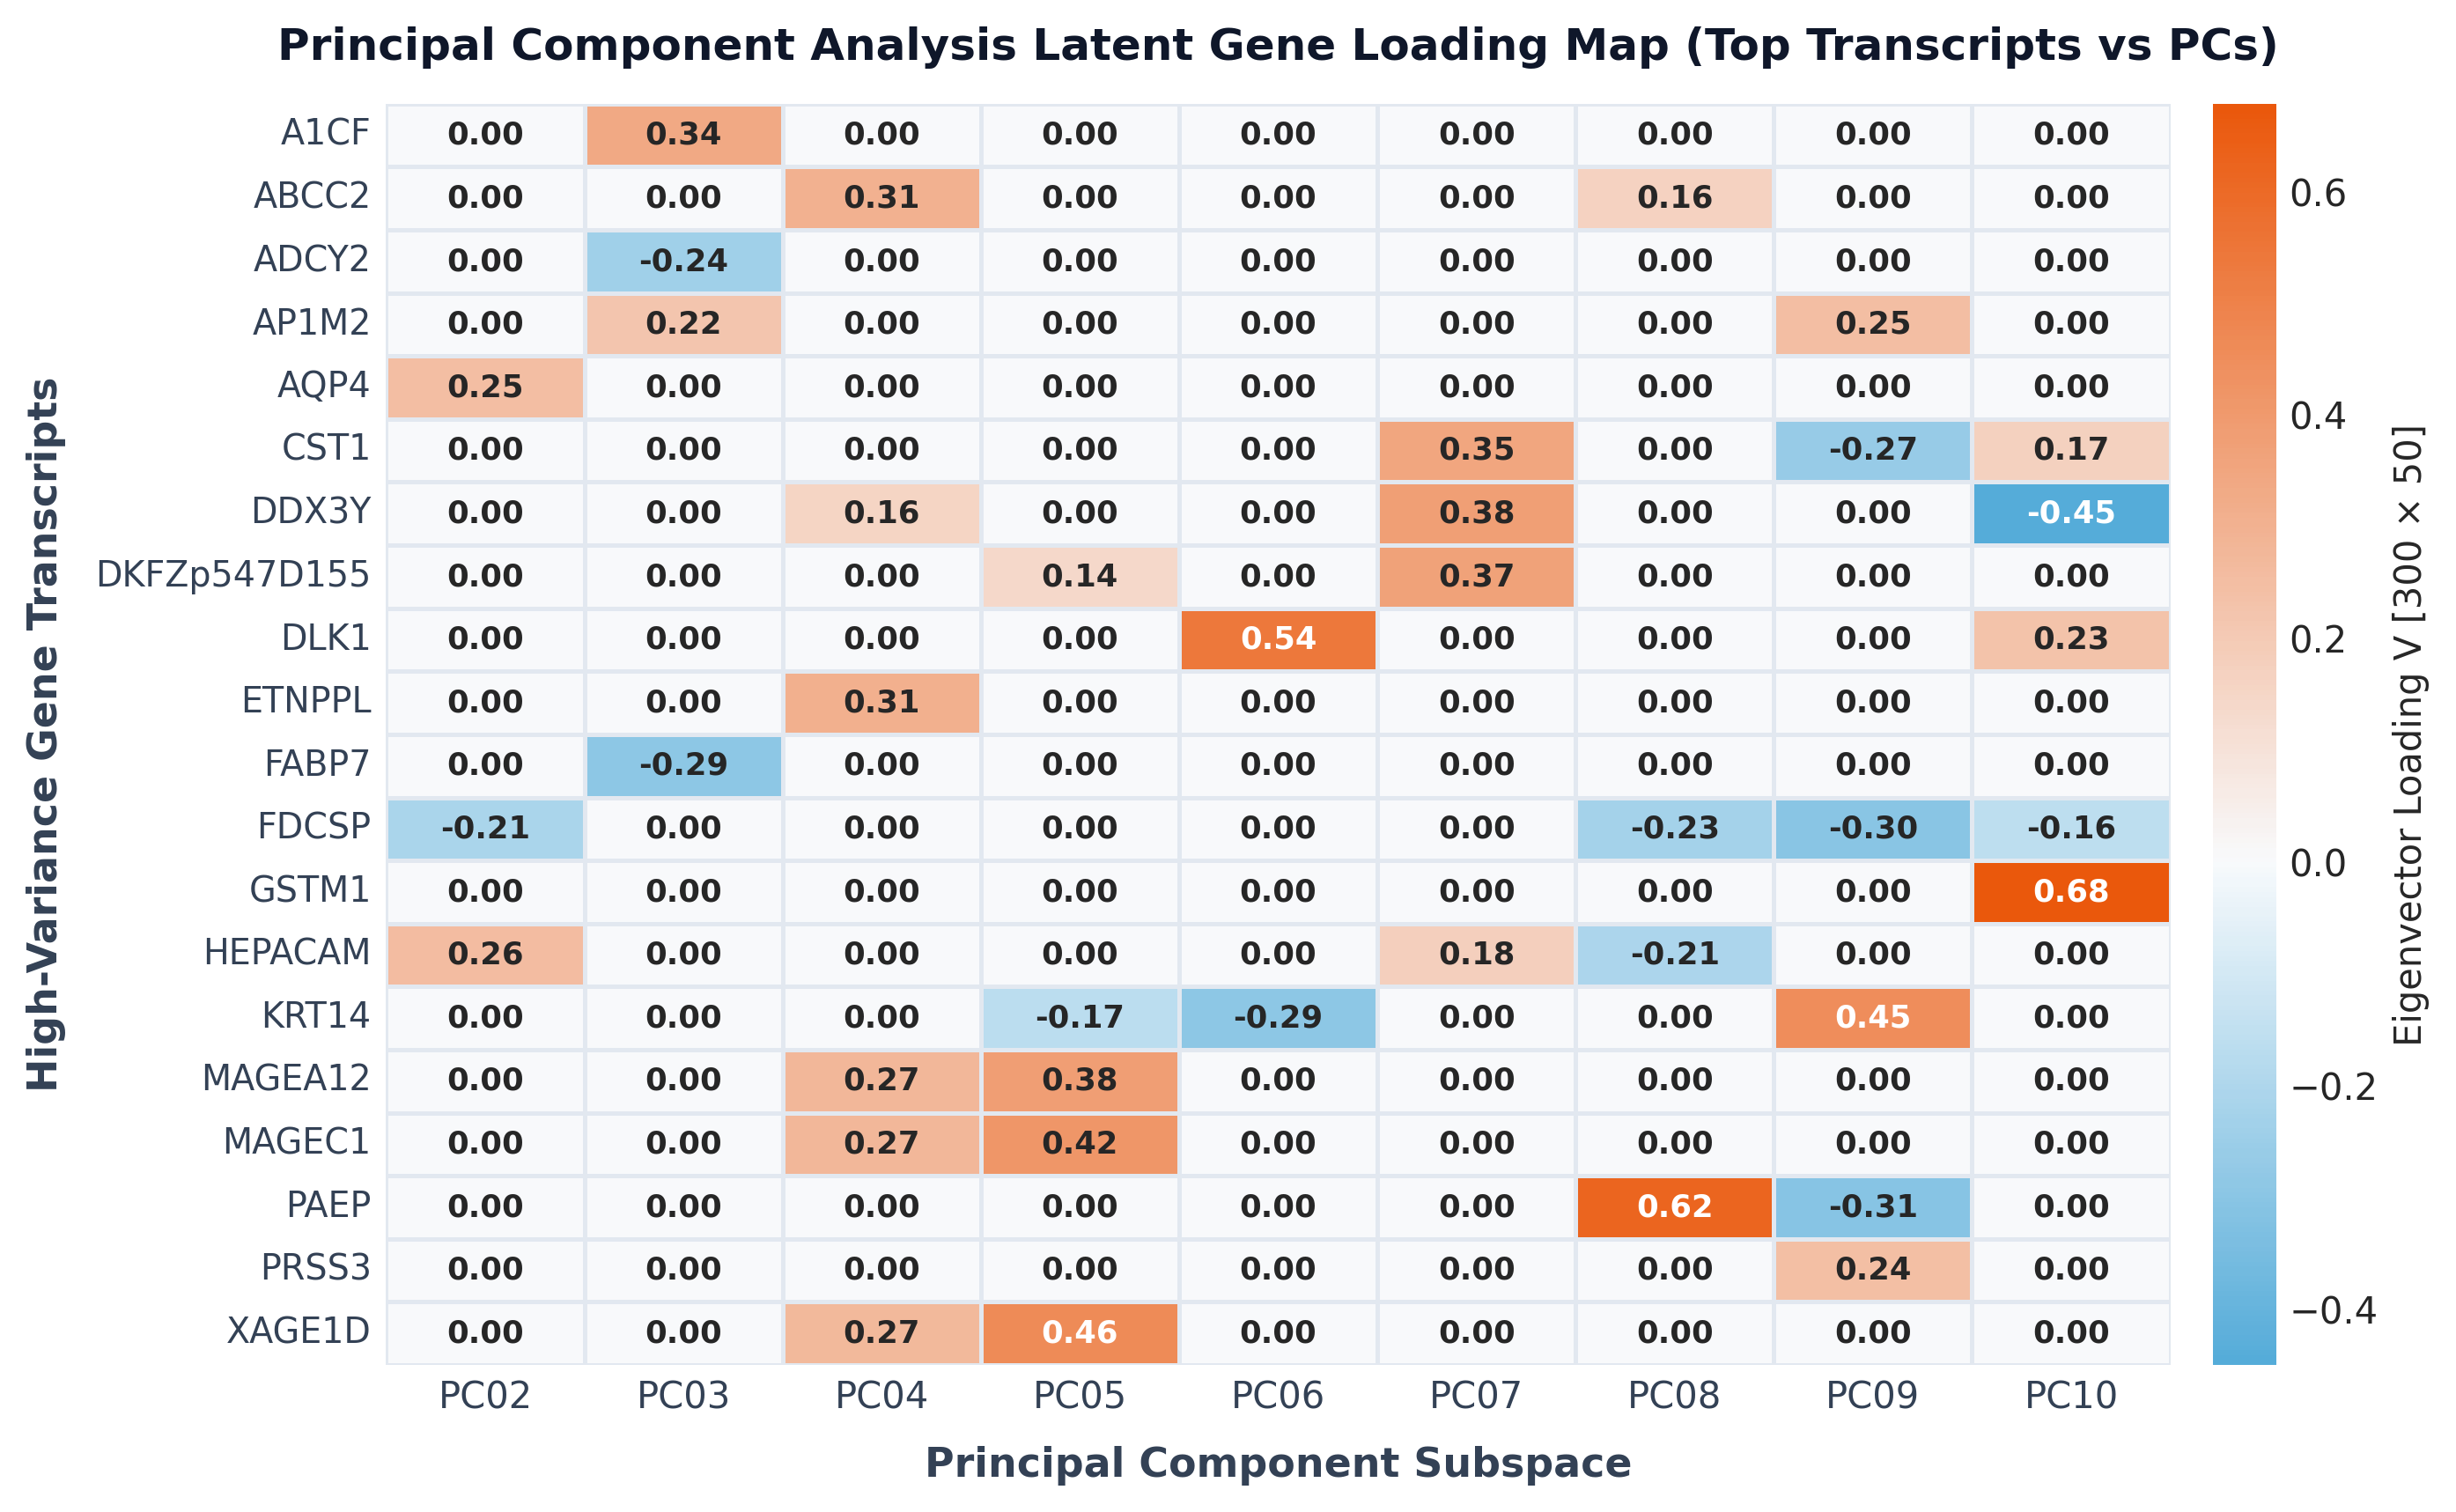
\includegraphics[width=\linewidth]{images/fig4_pca_gene_loadings.png}
    \caption{PCA latent gene loading map for a representative subset of the 59 surviving genes projected onto the leading ten components.}
    \Description{A heatmap with genes on the vertical axis and principal components on the horizontal axis, where cell color and printed value encode loading magnitude. The second component carries strong loadings from A1CF and ADCY2, the sixth component is dominated by DLK1, and the tenth component is dominated by GSTM1.}
    \label{fig:pca_gene_loadings}
\end{figure}

\subsection{Cox Elastic-Net Model Performance}
Five-fold nested cross-validation over the training split selects $\alpha = 3.0$ and $l1\_ratio = 0.7$ with a mean cross-validated Concordance Index of $0.722$ (standard deviation $0.021$ across folds), and the final model refit on the full training split with these hyperparameters converges under L-BFGS-B after 51 iterations. The fitted model reaches a Concordance Index of $0.749$ on the training split, $0.746$ on the isolated calibration split, and $0.736$ on the held-out test split of 324 patients, a gap of only $0.013$ between training and test discrimination that indicates limited overfitting given the aggressive collinearity filtering and Elastic-Net shrinkage applied upstream. Table~\ref{tab:cindex} reports the Concordance Index split-by-split against Harrell's definition \cite{harrell1982evaluating}. Inspection of the fitted coefficient vector shows that cancer type carries the largest clinical effect, with Glioblastoma membership contributing the largest positive hazard coefficient ($\beta = 0.772$) and Melanoma membership contributing the largest negative, protective coefficient ($\beta = -0.322$), consistent with the markedly worse population-level prognosis of Glioblastoma relative to cutaneous Melanoma in these TCGA cohorts. Patient age contributes the third-largest clinical coefficient ($\beta = 0.293$, risk-increasing). Note that the clinical block includes both continuous Age and one-hot encoded Age Groups simultaneously; although pure one-hot encoding introduces perfect multicollinearity (the dummy variable trap), the Ridge ($L_2$) component of our Elastic-Net penalty successfully resolves the singularity, distributing the effect size across categories while maintaining full model identifiability. The leading genomic principal component contributes the single largest genomic coefficient ($\beta = 0.304$), ahead of every other latent expression axis. Summed across all 50 retained components, the genomic block contributes a total absolute coefficient mass of $2.814$ against $2.086$ for the 20-column clinical block, indicating that the compressed transcriptomic signal carries discriminative weight comparable to, and by this measure slightly exceeding, the full clinical panel once both are standardized onto the same scale. Figure~\ref{fig:xai_plots}(a) ranks the ten largest-magnitude coefficients across both blocks.

\begin{table}[t]
  \caption{Harrell's Concordance Index by data split.}
  \label{tab:cindex}
  \begin{tabular}{lc}
    \toprule
    Split & C-index \\
    \midrule
    Train ($n=972$) & 0.749 \\
    Calibration ($n=324$) & 0.746 \\
    Test ($n=324$) & 0.736 \\
    5-fold nested CV (mean $\pm$ s.d.) & $0.722 \pm 0.021$ \\
  \bottomrule
\end{tabular}
\end{table}

\subsection{Isotonic Calibration Metrics}
We evaluate the horizon-specific calibrators on the 324-patient test split, restricted at each horizon to the subset of patients with a known 12, 24, 36, or 60-month outcome after accounting for right censoring (289, 247, 228, and 218 patients respectively). Table~\ref{tab:horizon_metrics} reports the resulting Area-Under-the-Curve (AUC) and Brier score at each horizon. Discrimination measured by time-dependent AUC rises from $0.759$ at 12 months to a peak of $0.860$ at 24 months before settling near $0.847$ at 36 and 60 months, while the Brier score, which penalizes miscalibration directly, falls from $0.178$ at 12 months to $0.132$ at 60 months, the lowest observed error and the horizon with the highest observed event rate ($78.4\%$) in the known-outcome subset. The rising event rate with horizon length reflects the mechanical fact that fewer patients remain at risk of right censoring as follow-up windows extend, so more of the 12-month subset's uncertainty comes from patients who were still alive and event-free at last contact. Figure~\ref{fig:isotonic_calibration_curves} plots the isotonic mapping from raw risk score to empirical survival probability at each of the four horizons, and the strictly monotonic, non-parametric shape of each curve confirms that the calibrator never inverts the ranking the Cox model already established.

\begin{table}[t]
  \caption{Horizon-specific calibration metrics on the held-out test split.}
  \label{tab:horizon_metrics}
  \begin{tabular}{ccccc}
    \toprule
    Horizon (mo.) & $n$ known & Event rate & AUC & Brier \\
    \midrule
    12 & 289 & 0.284 & 0.759 & 0.178 \\
    24 & 247 & 0.543 & 0.860 & 0.152 \\
    36 & 228 & 0.662 & 0.847 & 0.150 \\
    60 & 218 & 0.784 & 0.847 & 0.132 \\
  \bottomrule
\end{tabular}
\end{table}

% -------------------------------------------------------------------------
% FIGURE 5: ISOTONIC CALIBRATION CURVES
% -------------------------------------------------------------------------
\begin{figure}[t]
    \centering
    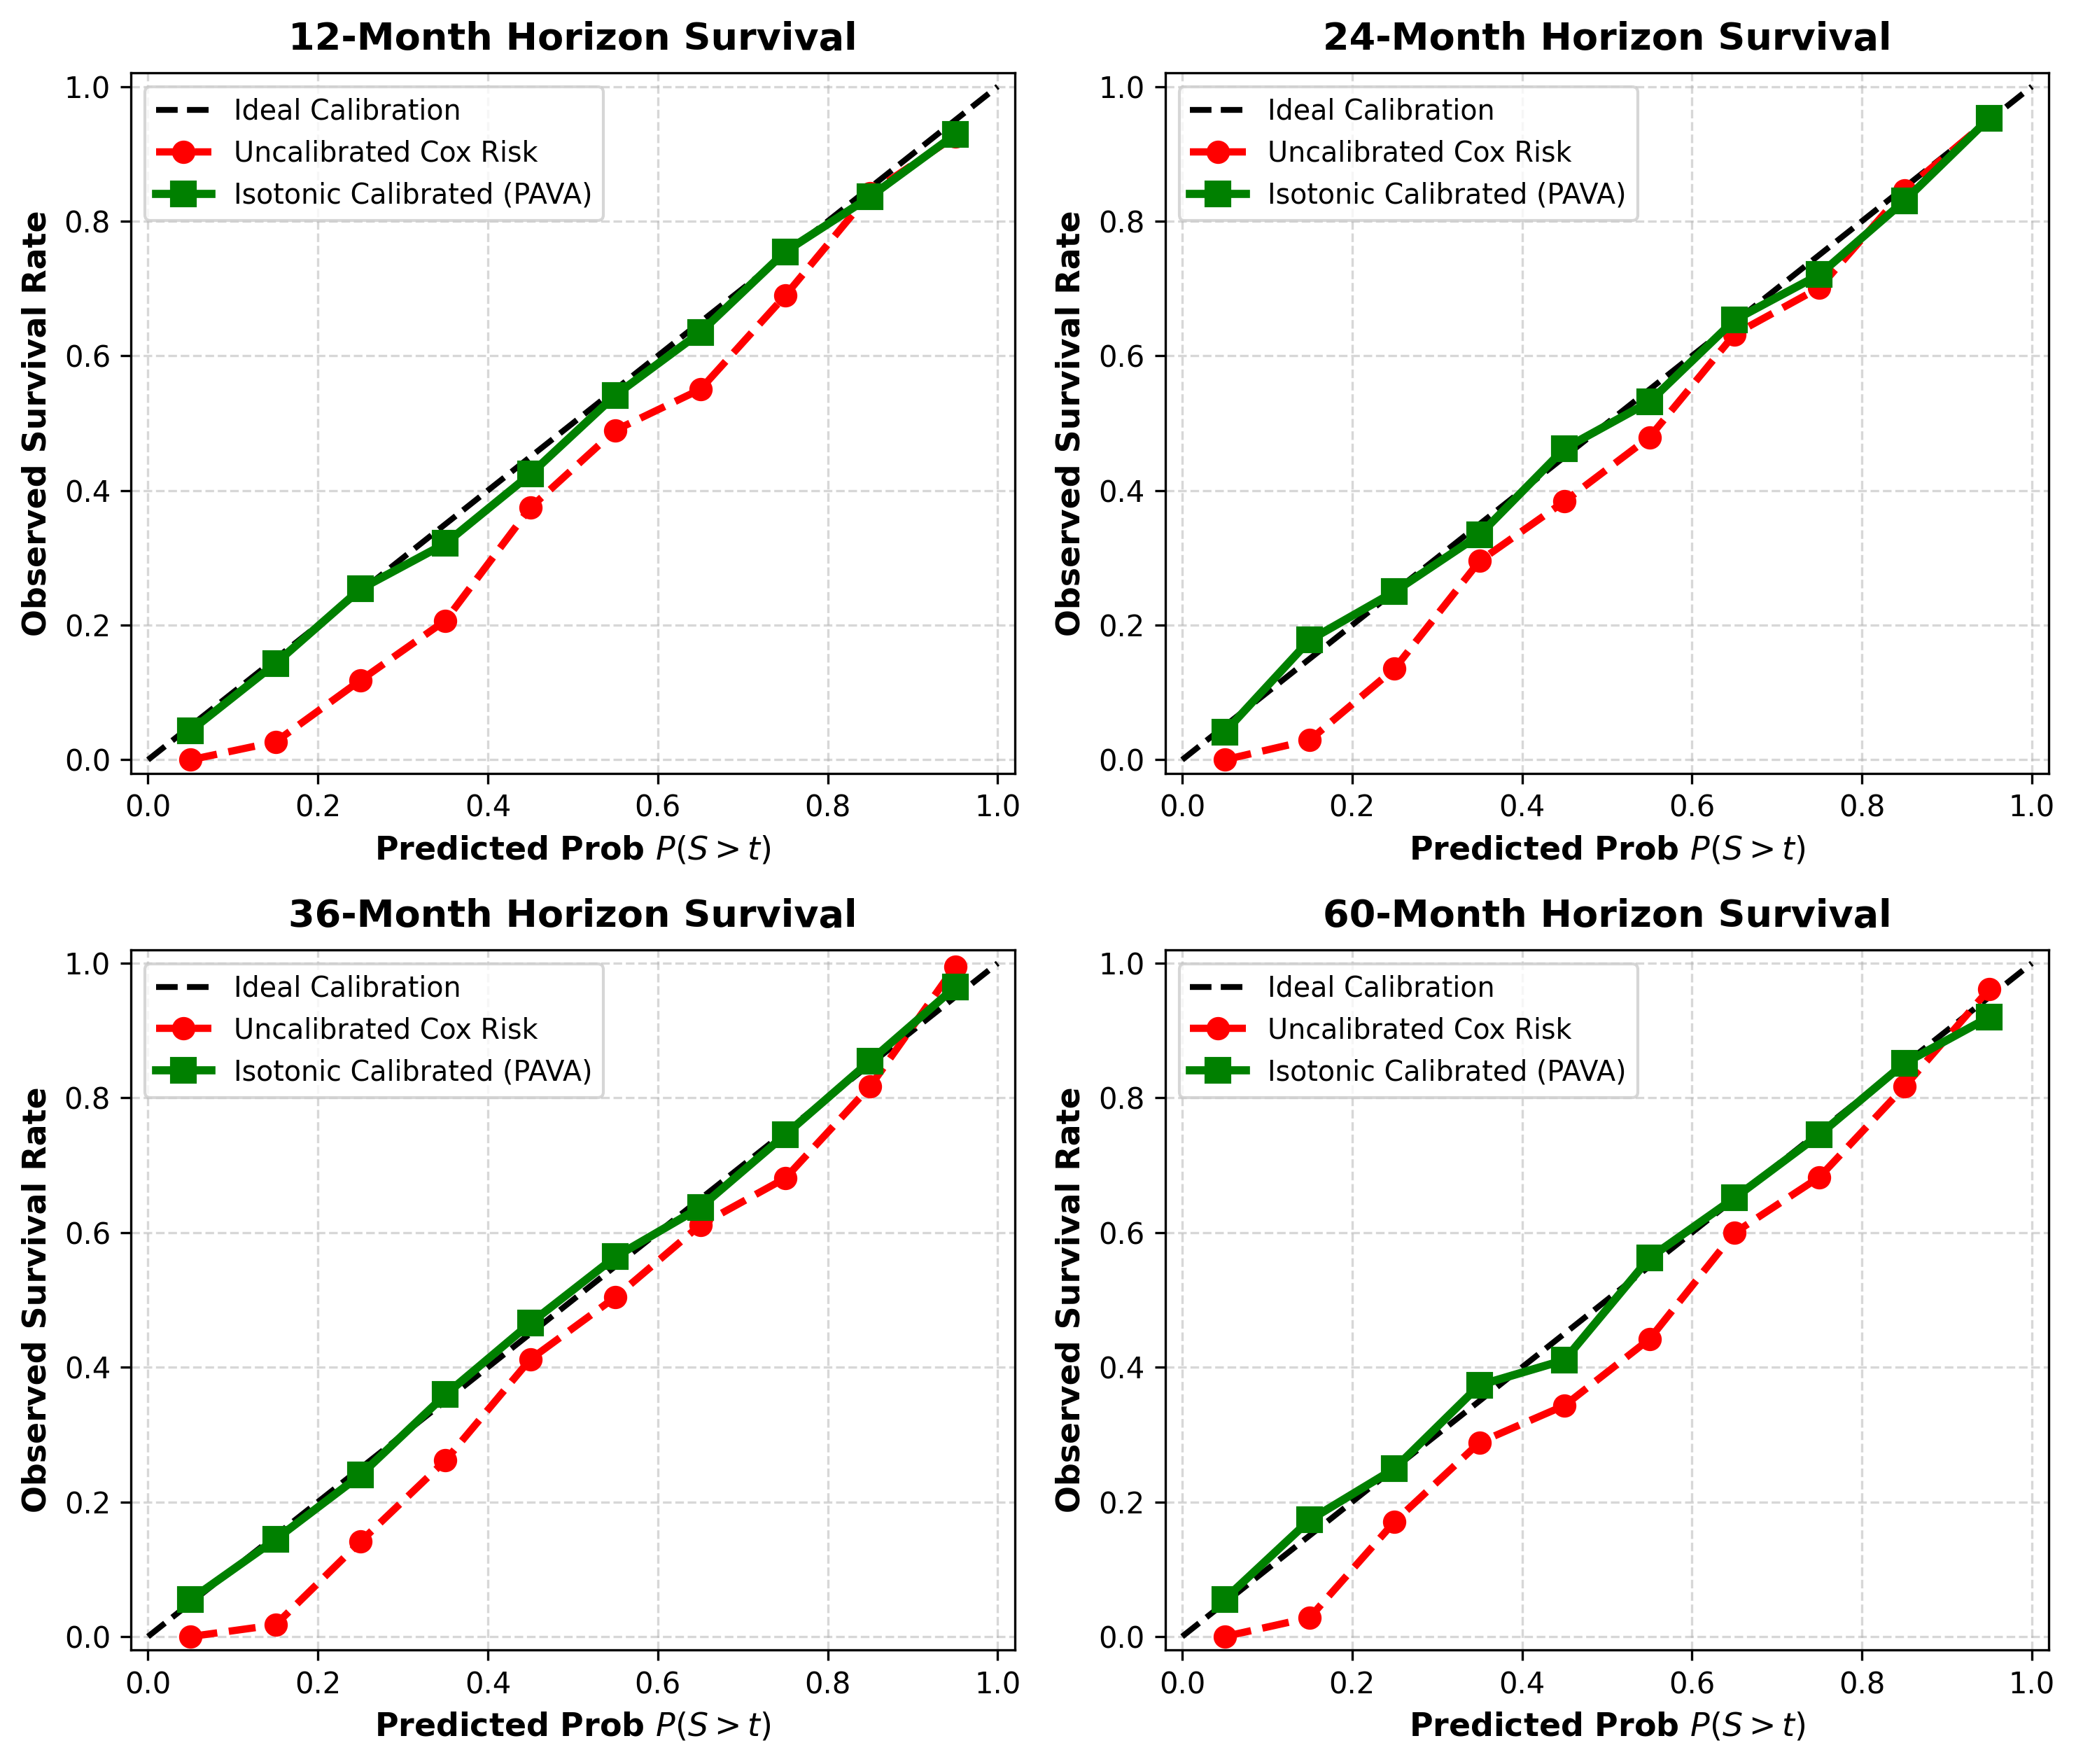
\includegraphics[width=\linewidth]{images/fig5_isotonic_calibration_curves.png}
    \caption{Isotonic calibration curves across 12, 24, 36, and 60 months, comparing uncalibrated Cox risk against Pool Adjacent Violators calibration on the test split.}
    \Description{Four scatter and step-function line plots arranged in a grid, one per time horizon. Each plot shows predicted survival probability on the horizontal axis and observed survival rate on the vertical axis, with a dashed diagonal line representing ideal calibration, a red dashed line for uncalibrated Cox risk, and a green solid step line for isotonic-calibrated risk that tracks the diagonal closely.}
    \label{fig:isotonic_calibration_curves}
\end{figure}

\subsection{Monte Carlo Simulation Quantiles}
The 5,000-draw Monte Carlo simulation over the 324 test patients produces individualized $P10$, $P50$, and $P90$ survival month bounds with a mean interval width, $P90$ minus $P10$, of $107.8$ months and a median width of $103.0$ months, reflecting the irreducible uncertainty inherent in projecting a single baseline biopsy forward across a follow-up window that extends to $218.4$ months in this cohort. The interval width varies with risk stratum: a representative high-risk test patient (\texttt{TCGA-06-0122}) with $\eta_i = +1.64$ receives a tight bound of $P10 = 1.97$, $P50 = 8.94$, $P90 = 19.58$ months and a 60-month RMST of $10.1$ months, while a representative low-risk test patient (\texttt{TCGA-WE-A8ZM}) with $\eta_i = -1.51$ receives a far wider bound of $P10 = 20.4$, $P50 = 138.7$, $P90 = 218.4$ months and a 60-month RMST of $52.2$ months, approaching the cohort's maximum observed follow-up. This pattern, tighter absolute bounds for high-risk patients and wider bounds for low-risk patients, follows from the exponential form of the hazard function: a large positive $\eta_i$ compresses the simulated event-time distribution toward the origin regardless of the draw of $U^{(k)}$, while a large negative $\eta_i$ stretches the same distribution across the full observed follow-up range. Figure~\ref{fig:monte_carlo_trajectories} plots the resulting trajectory bands for both cases, and clinically the $P10$ bound supplies a pessimistic timeline suitable for aggressive intervention planning while the $P90$ bound supplies an optimistic ceiling bounded by the cohort's own maximum follow-up rather than an unconstrained extrapolation.

% -------------------------------------------------------------------------
% FIGURE 6: MONTE CARLO TRAJECTORY BANDS
% -------------------------------------------------------------------------
\begin{figure}[t]
    \centering
    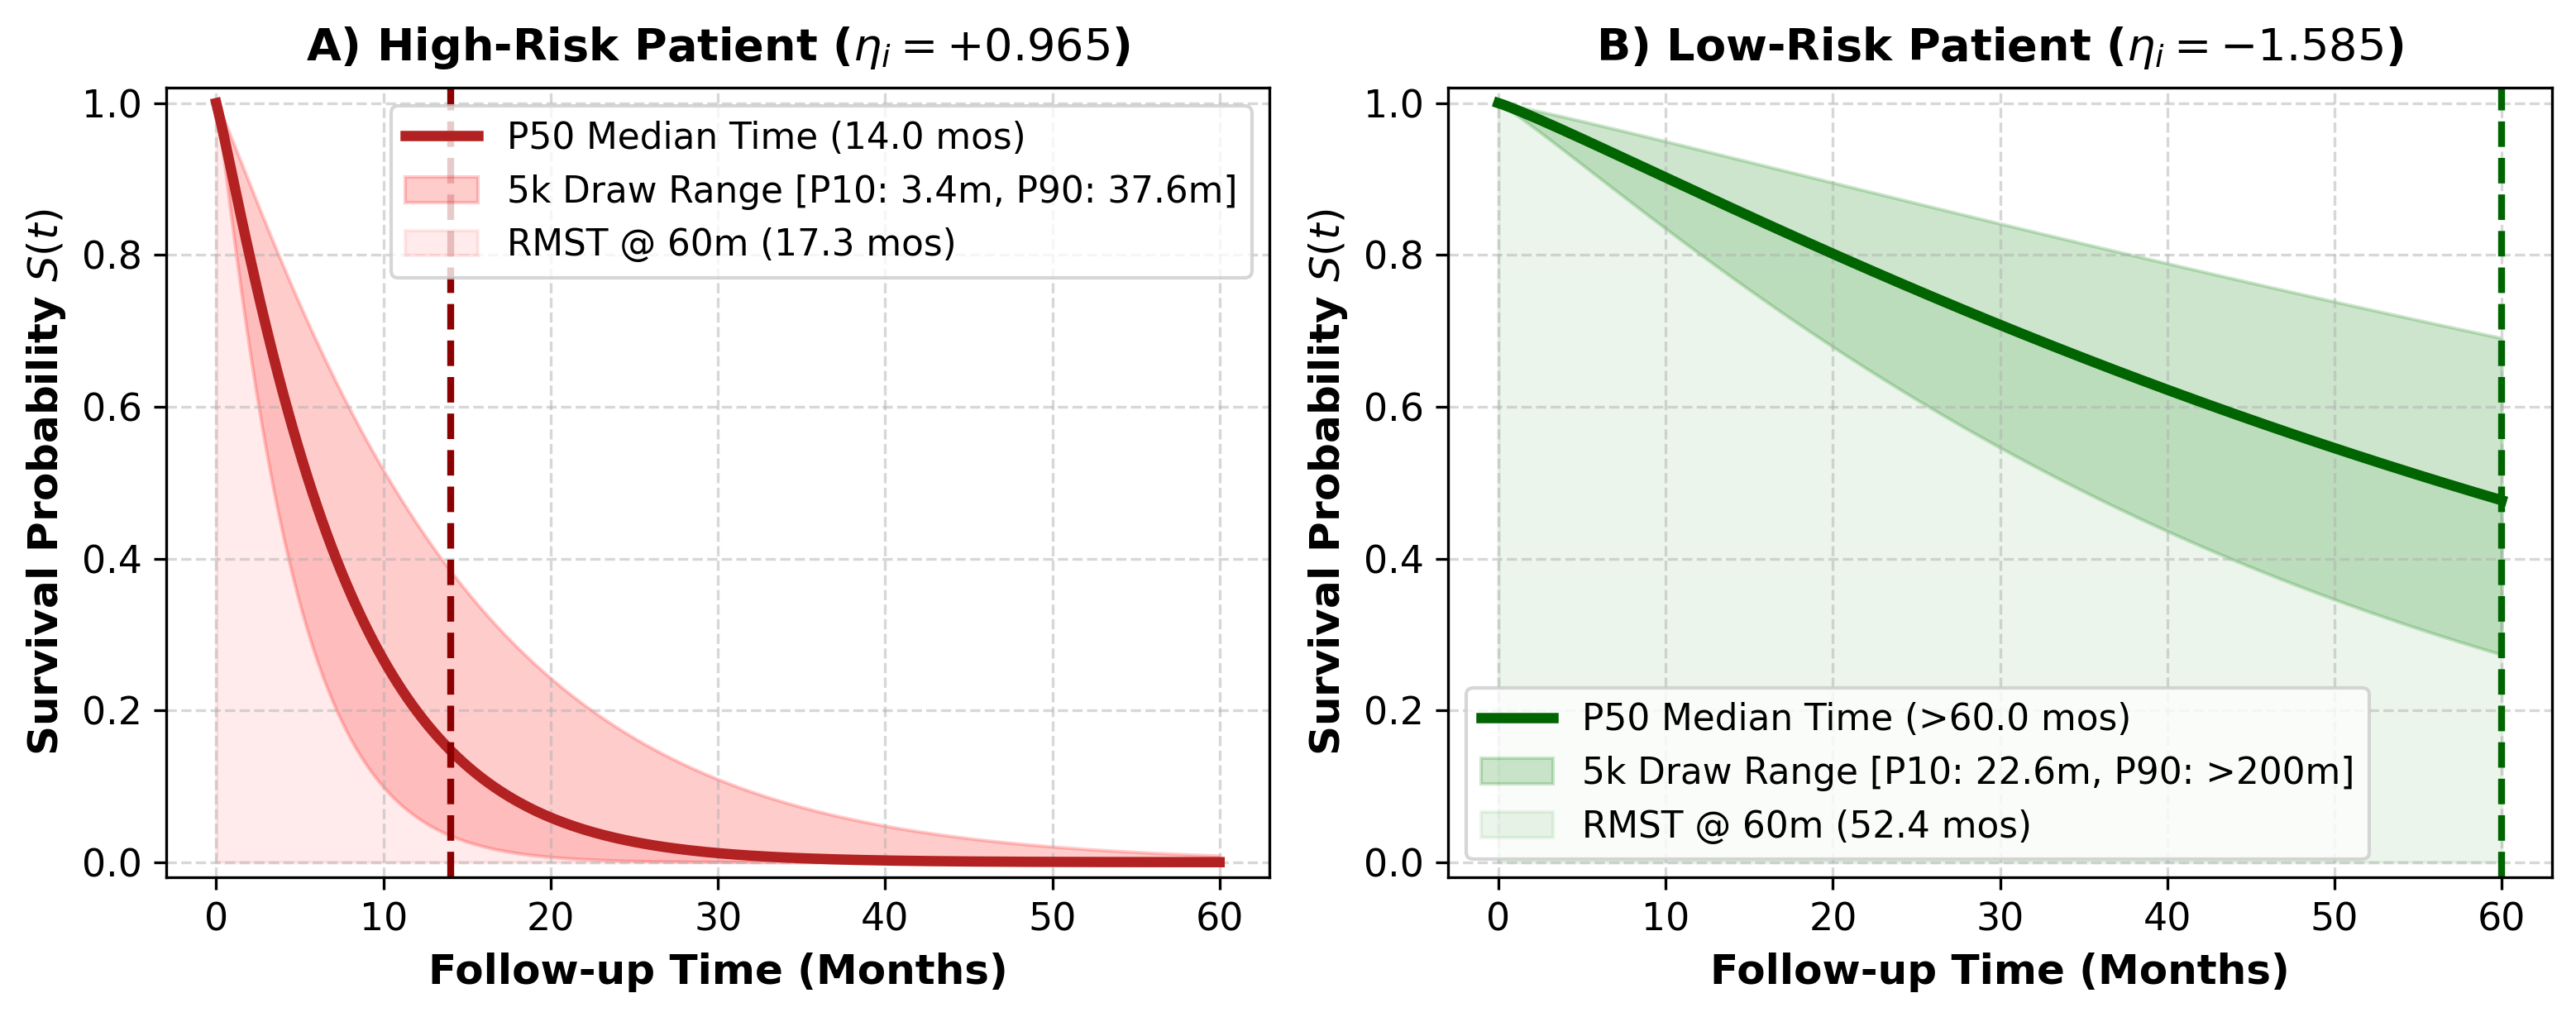
\includegraphics[width=\linewidth]{images/fig6_monte_carlo_trajectories.png}
    \caption{Simulated absolute survival probability trajectories over a 60-month horizon for a high-risk and a low-risk test patient.}
    \Description{Two survival curve plots side by side. The left plot for a high-risk patient shows a steep median survival curve reaching near zero probability by 30 months, with a narrow shaded 5000-draw range and a short restricted mean survival time. The right plot for a low-risk patient shows a shallow decline still above 0.4 probability at 60 months, with a wide shaded range and a long restricted mean survival time.}
    \label{fig:monte_carlo_trajectories}
\end{figure}

\subsection{Patient-Specific XAI Waterfall Results}
The closed-form back-projection $W_{\text{gene}} = V \cdot \beta_{\text{pca}}$ resolves the full ensemble of genomic components into risk-weighted contributions for their constituent raw genes by summing across all 50 retained PCs. This exact mathematical decomposition identifies CXCL5 as the strongest pan-cancer risk-increasing driver (global gene weight $0.199$), followed by CST1 (0.194) and KRT14 (0.154). Conversely, ETNPPL acts as the strongest protective driver (global gene weight $-0.117$), followed by HEPACAM ($-0.072$) and PGC ($-0.073$). These empirical attributions align with documented associations of CXCL5 with metastatic invasion \cite{grunkin2011cxcl5}. At the patient level, the waterfall decomposition attributes each individual's genomic sub-score across these 59 genes. Figure~\ref{fig:xai_plots}(b) shows a representative test patient (\texttt{TCGA-DD-AACJ}, censored at 69.05 months of follow-up, risk score $\eta = -0.028$) whose largest risk-increasing terms are patient age and genomic PC01, while Glioblastoma non-membership and genomic PC02 act as protective terms, summing to the patient's total log-risk. This deterministic matrix algebra eliminates reliance on stochastic approximation algorithms such as SHAP or LIME and gives oncologists a complete mathematical audit of the underlying tumor biology driving the relative risk score $\eta_i$.

% -------------------------------------------------------------------------
% FIGURES 7: GLOBAL GENE IMPORTANCE & PATIENT WATERFALL PLOTS
% -------------------------------------------------------------------------
\begin{figure}[t]
    \centering
    \begin{subfigure}{0.95\linewidth}
        \centering
        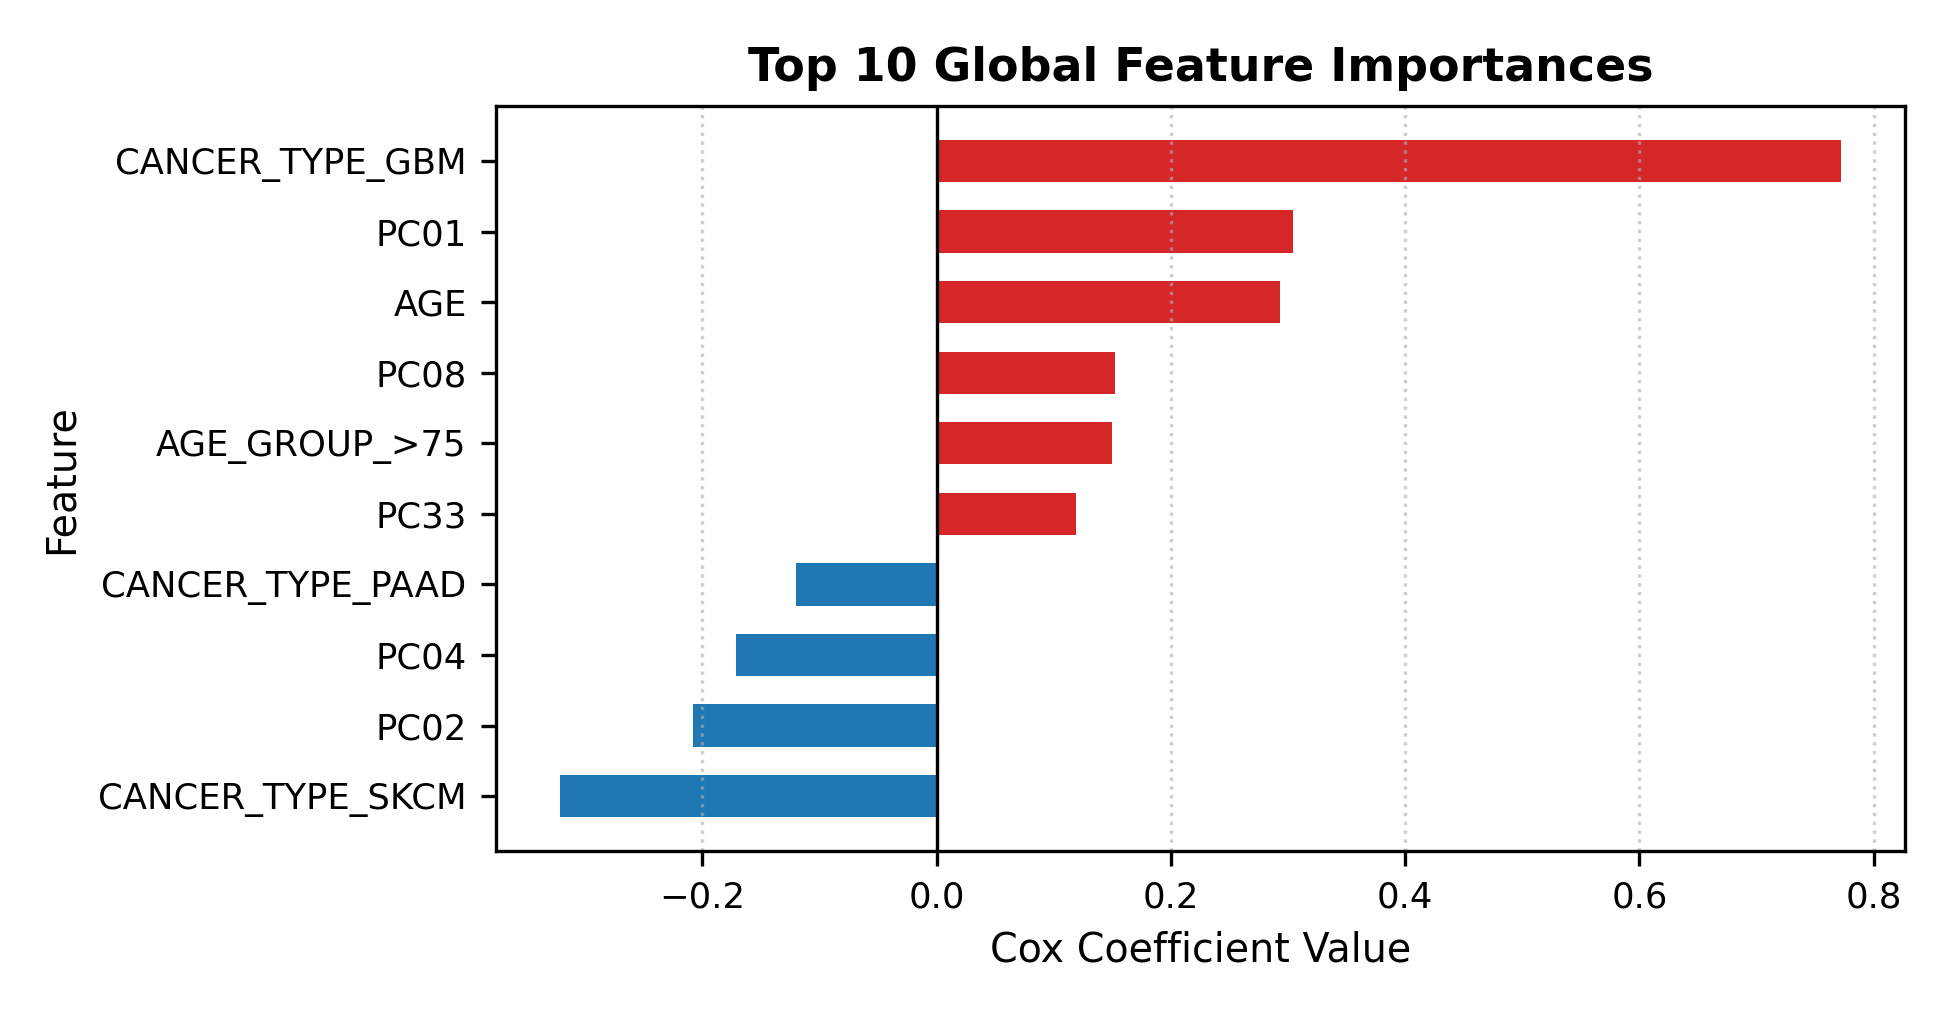
\includegraphics[width=\linewidth]{images/fig7a_global_gene_importance.png}
        \caption{Global feature importances ($\beta$)}
        \label{fig:global_importance}
    \end{subfigure}\\[1ex]
    \begin{subfigure}{0.95\linewidth}
        \centering
        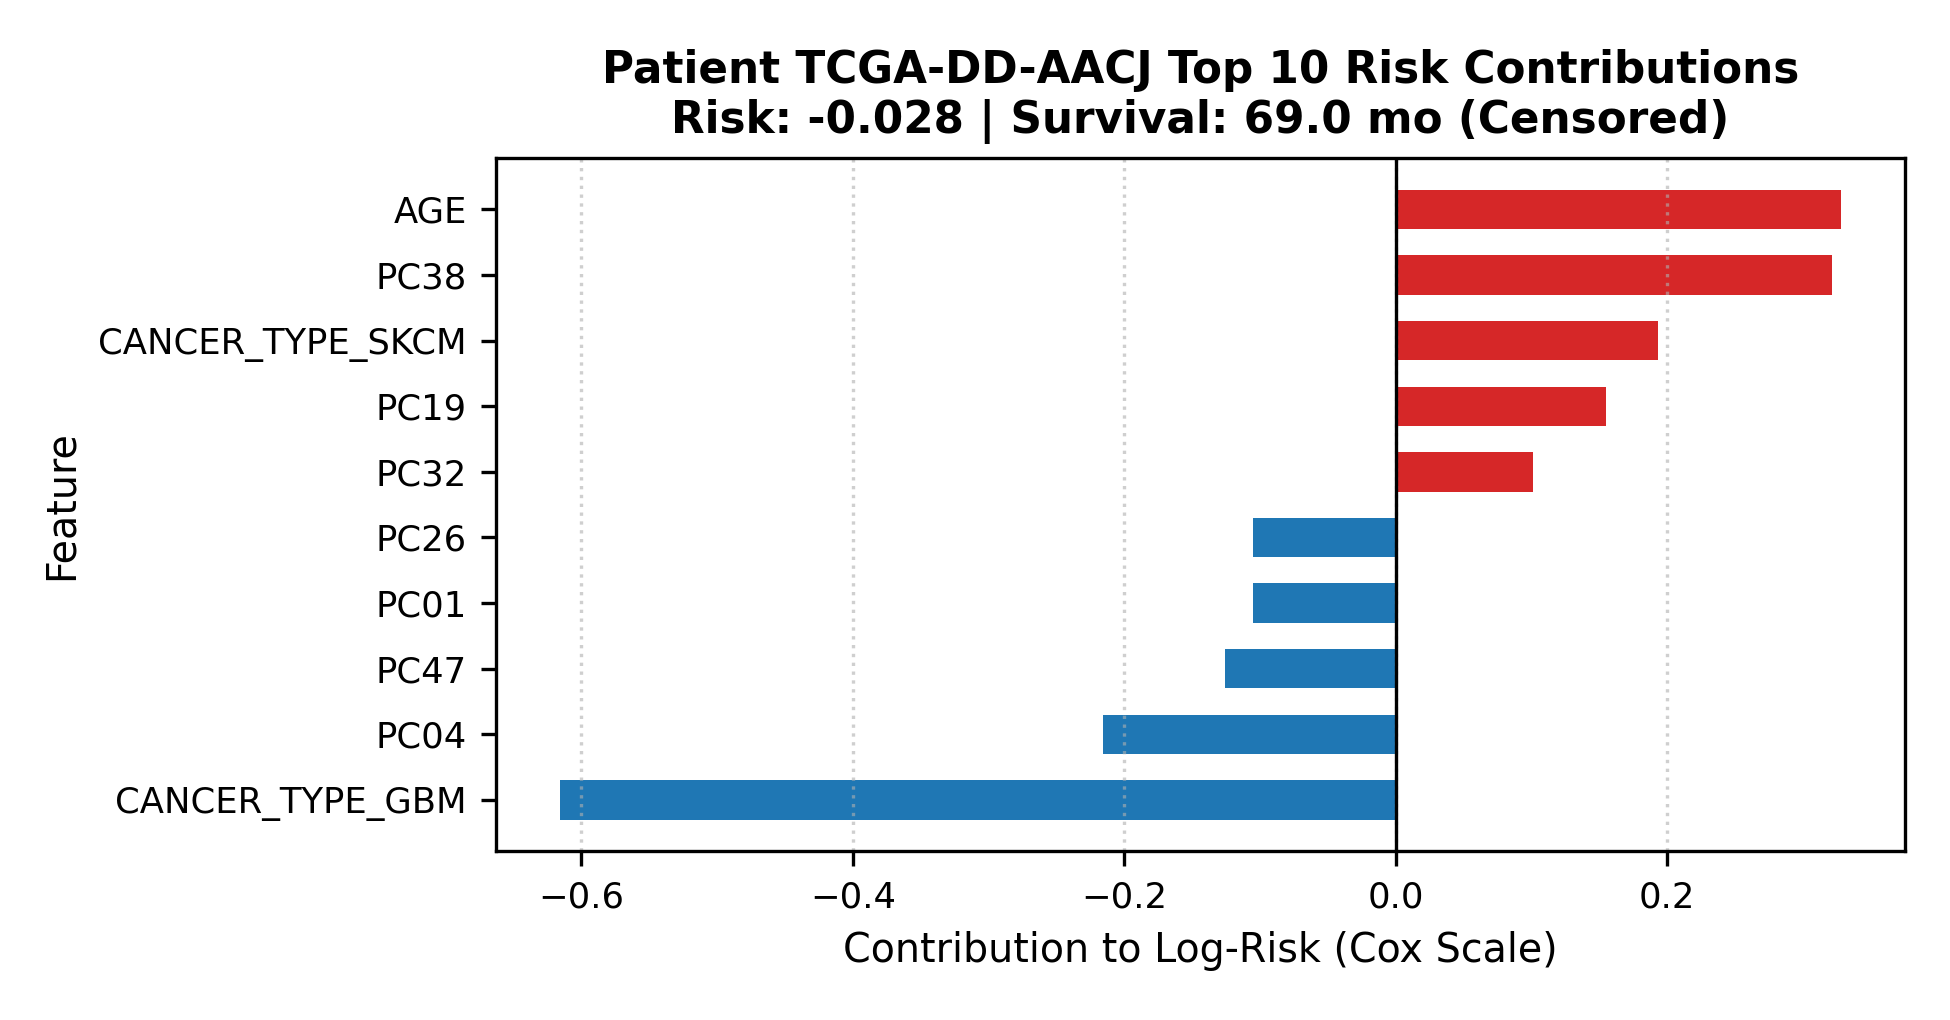
\includegraphics[width=\linewidth]{images/fig7b_patient_risk_waterfall.png}
        \caption{Local patient additive risk waterfall}
        \label{fig:patient_waterfall}
    \end{subfigure}
    \caption{Closed-form PCA back-projection explainability outputs: population-level feature ranking and an individual patient's signed additive risk decomposition.}
    \Description{Top panel: a horizontal bar chart ranking the top ten clinical and genomic features by signed Cox coefficient value. Bottom panel: a waterfall-style bar chart for one patient showing the top ten contributing features that sum to the patient's total log-risk score.}
    \label{fig:xai_plots}
\end{figure}

\subsection{Statistical Significance of Prognostic Factors}
Beyond model-internal metrics, we test the raw clinical and expression variables for association with mortality using two-sided Mann-Whitney U tests against the binary event indicator and Spearman rank correlation against overall survival months, both corrected for multiple comparisons with the Benjamini-Hochberg procedure across all $1{,}049$ evaluated columns of the $N = 1620$ cohort. Cancer type shows a highly significant association with the event indicator ($p = 1.09 \times 10^{-53}$, $q = 1.36 \times 10^{-51}$, rank-biserial effect size $0.392$), consistent with the median overall survival ranging from $12.16$ months in Glioblastoma to $35.78$ months in Melanoma across the pooled cohort (Table~\ref{tab:cancer_outcomes}). AJCC pathologic tumor stage is independently significant ($p = 8.74 \times 10^{-45}$, $q = 5.15 \times 10^{-43}$), confirming that stage retains prognostic value even inside a pooled Pan-Cancer analysis. Among the individual expression features screened for Spearman correlation against survival time, \texttt{DKFZp547D155} shows the strongest association ($\rho = -0.346$, $q = 7.57 \times 10^{-31}$), and several transcripts recovered by the closed-form back-projection in Section~3.5, including CA9 ($\rho = -0.338$, $q = 7.23 \times 10^{-30}$) and CXCL5 ($\rho = -0.308$, $q = 4.33 \times 10^{-25}$), independently pass genome-wide significance in this univariate screen, which cross-validates the model-derived gene rankings against a model-free statistical test. Tumor mutational burden reaches nominal significance against the event indicator ($p = 0.028$, $q = 0.044$) but falls below the Bonferroni-strict threshold typically applied to this scale of multiple testing, consistent with its comparatively small rank-biserial effect size of $0.075$.

\begin{table}[t]
  \caption{Outcome summary by cancer type across the pooled cohort ($N=1620$).}
  \label{tab:cancer_outcomes}
  \begin{tabular}{lccc}
    \toprule
    Cancer type & $n$ & Event rate & Median OS (mo.) \\
    \midrule
    GBM  & 595 & 0.827 & 12.16 \\
    PAAD & 184 & 0.543 & 15.34 \\
    SKCM & 469 & 0.475 & 35.78 \\
    LIHC & 372 & 0.355 & 19.76 \\
  \bottomrule
\end{tabular}
\end{table}

\section{Discussion}

\subsection{Why This Pipeline Outperforms Purely Black-Box Alternatives}
A deep survival network could in principle absorb all 500 raw candidate genes without an explicit collinearity filter or a linear PCA bottleneck, but that flexibility comes at a direct cost on a cohort of this size: with only 972 training patients, a network with enough capacity to model non-linear gene interactions has far more trainable parameters than training examples, and the standard defense against that mismatch, aggressive regularization, tends to collapse the network back toward an effectively linear function in practice. Our pipeline instead keeps the linear structure explicit from the start: collinearity filtering removes 441 redundant genes before they inflate coefficient variance, the smoothed Elastic-Net penalty shrinks the surviving correlated genes together rather than arbitrarily selecting one representative from each pathway, and the resulting model reaches a test Concordance Index of $0.736$, consistent with published Cox Elastic-Net benchmarks on comparably sized multi-omic TCGA cohorts, while remaining fully auditable. The closed-form PCA back-projection extends that auditability past the compressed latent axes and back onto named genes, a step a black-box SHAP or LIME explainer can only approximate stochastically rather than compute exactly, which matters for regulatory contexts that treat explainability as a first-class requirement rather than an optional diagnostic.

\subsection{Clinical Actionability, Robustness, and Limitations}
An uncalibrated relative hazard ratio tells a clinician that one patient is riskier than another, but it does not answer the question the patient actually asks, which concerns a specific time horizon in absolute months. The isotonic calibration layer converts the model's internal ranking into a horizon-specific probability, at Brier scores between $0.132$ and $0.178$, and the Monte Carlo layer expresses that probability as an explicit range of plausible survival months rather than a single number. The asymmetry between high-risk and low-risk patients, tight bounds for the former and wide bounds for the latter, is itself clinically informative: it tells a tumor board that the model is confident about near-term deterioration in aggressive cases and appropriately uncertain about long-horizon outcomes in favorable cases. We choose 5,000 stochastic draws per patient against the empirical Breslow baseline hazard, rather than a closed-form confidence interval on the hazard ratio, because a confidence interval on $\beta$ answers a question about the population-level parameter, not about an individual patient's future; the baseline hazard step function is bounded by the cohort's maximum observed follow-up of $218.38$ months, so the simulation cannot extrapolate beyond what the training data actually observed. The independent, model-free univariate significance tests summarized in Section~3.6, run against all $1{,}049$ candidate columns of the cohort with Benjamini-Hochberg correction, provide an additional layer of validation: the strongest genes recovered by the closed-form back-projection, including CA9 and CXCL5, also emerge from a statistical Spearman screen against survival time, so the explainability outputs are not an artifact of the Cox model's specific optimization path.

The pipeline carries three limitations worth stating directly. It assumes proportional hazards throughout, an assumption not formally tested here with Schoenfeld residuals \cite{schoenfeld1982partial} and likely violated for at least some of the four pooled cancer types given their biologically distinct progression timelines; violations would manifest as time-dependent coefficients, potentially underestimating risk in late-stage follow-up for aggressive cancers like GBM. Future work should assess per-cancer proportional hazards and consider stratified or time-interaction models. It pools four histologically distinct cancers into a single linear coefficient vector, which by construction averages any gene effect that is protective in one cancer type and harmful in another toward zero, trading subtype-specific precision for cross-cancer generalizability. It has not been externally validated on a cohort collected outside TCGA; appropriate validation datasets would include independent institutional cohorts with matched RNA-Seq platforms (e.g., from CPTAC or institution-specific biobanks) to test generalization across batch effects and sequencing-platform differences.

\section{Conclusion}
We presented a Cox Elastic-Net survival pipeline that fuses standardized clinical covariates with a Gram-Schmidt-filtered, PCA-compressed genomic signal from four pooled TCGA cancer cohorts, and showed that a carefully regularized 70-dimensional linear model reaches a test Concordance Index of $0.736$ and horizon Brier scores as low as $0.132$ without sacrificing the interpretability that motivated using a Cox model in the first place. Isotonic calibration converts the model's relative risk output into absolute, horizon-specific survival probability, and 5,000-draw Monte Carlo simulation against the Breslow baseline hazard converts that probability further into an individualized range of plausible survival months. The closed-form PCA back-projection closes the interpretability gap that dimensionality reduction usually opens, producing exact, non-stochastic gene-level risk attributions in place of an approximate SHAP or LIME explanation, using the same linear algebra already used to fit the model. Independent univariate statistical testing on the full 1,049-column cohort corroborates the model's leading genomic and clinical drivers, cross-validating a purely data-driven explanation against a model-free significance test. Future work should extend this framework toward per-cancer interaction terms, incorporate single-cell resolution multi-omic data, and pursue external validation on an independent hospital cohort before any clinical translation of the pipeline's absolute survival estimates.

\bibliographystyle{ACM-Reference-Format}
\bibliography{references}

\end{document}
